\documentclass[runningheads]{llncs}

\usepackage[T1]{fontenc}
\usepackage{graphicx}
\usepackage{hyperref}
\usepackage{amsmath,amssymb}
\usepackage{setspace}
\usepackage{etoolbox}
\usepackage{enumitem}

\newcommand{\ms}[1]{\ensuremath{\mathsf{#1}}}
\newcommand{\msi}[1]{\ensuremath{\mathsfit{#1}}}

\begin{document}

\title{A Decentralized Mnemonic Backup System\\ for Non-Custodial Cryptocurrency Wallets}
\titlerunning{A Decentralized Mnemonic Backup System}

\author{Thierry Sans\inst{1,3} \and
(David) Ziming Liu\inst{2,3}\and
Kevin Oh\inst{3}}

\institute{University of Toronto Scarborough, Toronto, Canada \and dApp Technology Inc. Toronto Canada \and PriFi Labs Inc. Toronto, Canada \\[2ex] \email{thierry.sans@utoronto.ca} \makebox[1em]{} \email{david.liu@dapp-inc.com} \makebox[1em]{} \email{kevin.oh@prifilabs.com}}

\maketitle             

\begin{abstract}

When using non-custodial cryptocurrency wallets such as Exodus (Bitcoin), Metamask (Ethereum), and Keplr (Osmosis), the private keys are directly stored on the user's device. Using such a wallet comes with the risk of losing all crypto assets when the device gets lost, stolen, or breaks down irremediably. Fortunately, most non-custodial wallets offer a way to recover the private keys by the mean of a ``recovery phrase'' also known as a ``mnemonic seed phrase''. It is the 12-word phrase that is given when the wallet is created. Indeed, this mnemonic phrase is a really sensitive piece of information since anyone knowing that phrase can get full control of the crypto assets held by the wallet. Usually, it is recommended to write this passphrase down on a piece of paper and store it in a “safe place”. However, storing a physical object is still not ideal since it can get stolen, lost, or destroyed as well. In this paper, we propose a decentralized application that can be used to back up mnemonic phrases and recover them eventually using a simple email. This application is built on a privacy-preserving blockchain to store the confidential passphrase and protect the identity of its owner.

\keywords{Blockchain  \and Smart Contracts \and Decentralized Applications \and Privacy \and Wallets \and Cryptography Protocol}
\end{abstract}

\section{Introduction}

In the world of cryptocurrency, a {\em wallet} provides users with an interface to manage their crypto assets. Under the hood, those wallets store a set of private keys and use them to sign transactions. There are two types of wallets: ``custodial wallets'' in which the private keys are in the custody of a trusted third party and ``non-custodial wallets'' in which the private keys are directly stored on the user's device whether it is a computer, a mobile phone or a dedicated USB dongle. Using either of these types of wallets comes with inherent risks \cite{azar2022financial}. Using custodial wallets comes with the risk of losing all crypto assets when the trusted entity goes bankrupt\footnote{as popularized by the mantra from {\em Andreas Antonopoulos}: {\em ``Not Your Keys, not Your Coins''}} and non-custodial wallets come with the risk of losing all crypto assets if the device gets lost, stolen or irremediably breaks down. \\

Yet, non-custodial wallets (our focus here) such as Exodus (Bitcoin), Metamask (Ethereum), and Keplr (Secret Network) offer a way to recover the private keys through the mean of a ``recovery phrase'' also known as ``mnemonic seed phrase''. It is the 12-word phrase given the first time a wallet is set up. Here is an example of such a phrase: 

\begin{quote}
\begin{center}
{\tt witch fox practice feed shame open}\\
{\tt despair creek road again ice least}
\end{center}
\end{quote}

That phrase is important as it is used to generate the same private keys on demand (BIP39 standard \cite{palatinus2013mnemonic}). It can be used as a backup or to import the wallet into a new device. Indeed, this mnemonic phrase is a really sensitive piece of information. Anyone who has access to this phrase would have full control over the crypto assets as explained in the {\em Metamask} Wallet FAQ page:

\begin{quote}
{\em ``MetaMask requires that you store your Secret Recovery Phrase in a safe place. It is the only way to recover your funds should your device crash or your browser reset. We recommend you to write it down. The most common method is to write your 12-word phrase on a piece of paper and store it safely in a place where only you have access. Note: if you lose your Secret Recovery Phrase, MetaMask can’t help you recover your wallet. Never give your Secret Recovery Phrase or your private key(s) to anyone or any site, unless you want them to have full control over your funds.''}\\
\end{quote}

As written above, users are not supposed to remember that phrase like a password but instead write it down on a piece of paper and store it in a ``safe place''. However, storing physical objects is still not ideal since they can get stolen, lost, or destroyed as well. As a consequence, users do not always follow such a recommendation and put themselves at risk as studied in \cite{voskobojnikov2021u}. So, as an alternative, could we design a simple application that would take custody of that passphrase and would allow users to recover it based on some sort of authentication? Intuitively, that application could be something similar to a password manager but such a solution requires 1) that the service provider is trustworthy and 2) that the whole application is secured \cite{li2014emperor}. Moreover, a password manager is a centralized solution that goes against the idea of decentralized applications \cite{buterin2017ethereum,cai2018decentralized}. \\

In this paper, we propose a decentralized application that can be used to back up private keys and mnemonic phrases and recover them eventually using a simple email. This application is built on a privacy-preserving blockchain \cite{zyskind2015decentralizing} to store the confidential passphrase and protect the identity of its owner. To better explain our idea, we will go through 3 iterations each more secure than the previous one. In the first iteration (section \ref{iteration1}), we aim at capturing the user experience but its overall design is rather naive and not secure. In the second iteration (section \ref{iteration2}), we harden the security by encrypting the passphrase and separating the key storage from the passphrase storage. That second iteration makes use of Non-Fungible Tokens (NFT) \cite{wang2021non} and the well know {\em Diffie–Hellman key exchange protocol} \cite{diffie2022new} to securely generate the encryption key directly on the blockchain. Finally, in the third iteration (section \ref{iteration3}), we improve the reliability by splitting and distributing the encrypted passphrase across the network using another cryptographic protocol called {\em Shamir's Secret Sharing scheme} \cite{shamir1979share}. 

\section{Iteration 1: The User Experience}
\label{iteration1}

Alice is a blockchain user that holds all kinds of crypto assets using different wallets. She would like to have an online backup of all of her wallet's passphrases in case her device gets lost, stolen, or breaks down irremediably. When that doomsday comes, she would like to recover her passphrases easily. The overall user experience is rather simple: 

\begin{itemize}
    \item {\bf When Alice wants to back up a passphrase}, she visits our Mnemonic Backup website and enters a passphrase and her email. After submitting her information, our application sends her an email with a confirmation code that she must copy onto the webpage to finalize the backup process. 
    \item {\bf When Alice wants to recover a passphrase}, she visits our Mnemonic Backup website and enters her email. Our application sends her an email with a verification code that she must copy onto the webpage before getting her passphrase back. 
\end{itemize}

This user experience is similar to existing security mechanisms used in traditional web applications where we must make sure that the user is the legitimate owner of the email address used for signing up, signing in (with two-factor authentication enabled), or reseting a password.

\subsection{Architecture}

Our Mnemonic Backup System is a decentralized application developed and deployed on a privacy-preserving blockchain called {\em Secret Network} \cite{zyskind2015decentralizing}. Secret Network Smart Contracts enable storing and processing of private data directly on the blockchain. It relies on the Intel SGX (Software Guard Extension) Trusted Execution Environment (a.k.a Confidential Computing) \cite{mckeen2013innovative} to prevent validator nodes from reading private data directly from memory during execution. \\

For this first iteration, we implement our Mnemonic Backup System as a smart contract on the Secret Network that records the passphrase when backing up and restores that passphrase when recovering. However, our secret contract cannot send emails by itself, so we are pairing it with an off-chain Mailer Backend that will send emails to users. So, there are three entities in our system:

\begin{itemize}
    \item {\bf The Backup Contract} is the smart contract that stores users' email and passphrases (the first iteration only, it will change in our second iteration)
    \item {\bf The Frontend Client} is the webpage that allows users to back up and recover passphrases.
    \item {\bf The Mailer Backend} is the off-chain mailer that sends confirmation/verification codes the users. For security reasons, the mailer backend never handles any passphrase. Only the Backup Contract has access to passphrases.
\end{itemize}

\subsection{The Protocol}

{\bf For backup} (see figure~\ref{it1:backup}), the goal is to verify Alice's email address to eventually store her passphrase. 

\begin{figure}[t]
  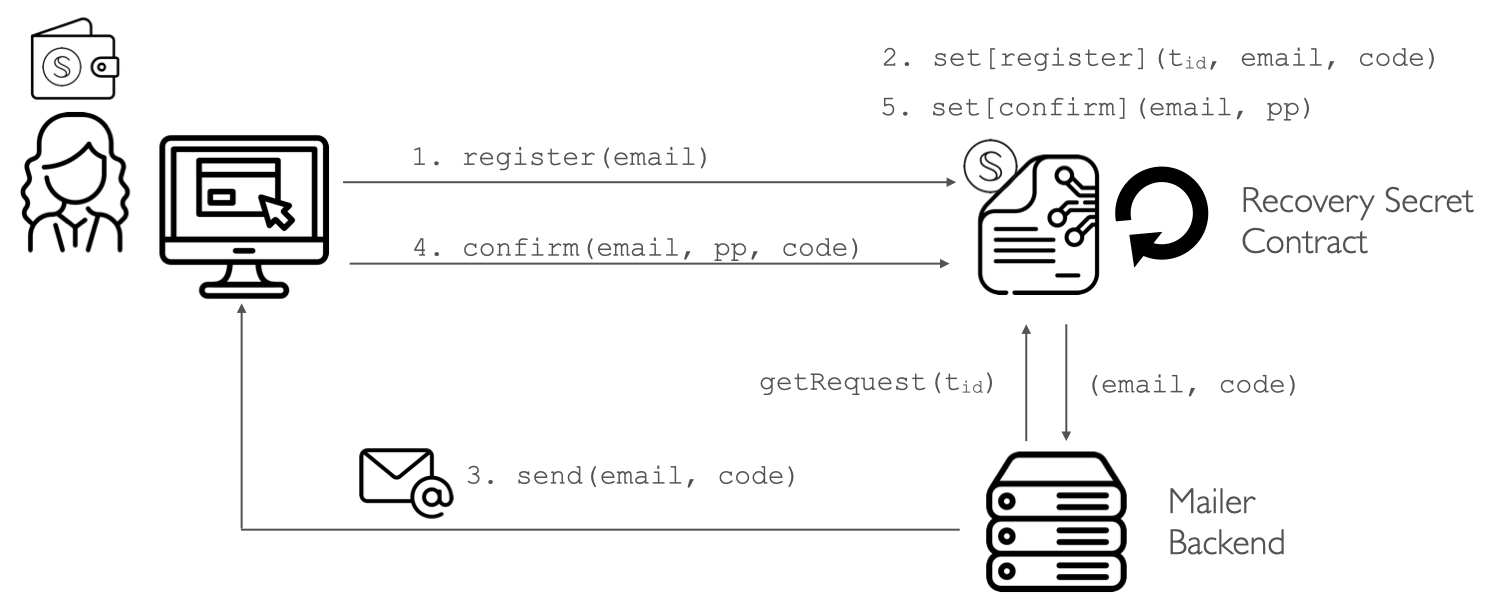
\includegraphics[width=\linewidth]{./media/media-001.png}
  \caption{Iteration 1 - Backup}
  \label{it1:backup}
\end{figure}

\begin{enumerate} 
\item Alice enters her $email$ and, after pressing the submit button, a script running inside the webpage sends a transaction {\bf $\ms{register}(email)$} to the Secret Network using a throwaway Secret wallet that Alice has just provisioned. 
\item The Backup Contract generates a transaction id $t_{id}$, a random confirmation code, stores the record $(t_{id}, email, code)$ in the {\tt register} dataset, and returns the transaction id to Alice.
\item Alice forwards the transaction id to the Mailer Backend. 
\item The Mailer Backend queries the Backup Contract using that transaction id. 
\item The Backup Contract returns the email and confirmation code associated to the transaction id. 
\item The Mailer Backend sends the confirmation code to Alice by email. 
\item Alice opens her email and copies and pastes the confirmation code into her browser and her passphrase $pp$. After pressing the submit button, a script, running inside the webpage, sends a transaction $\ms{confirm}(email, pp, code)$ to the Backup Contract. 
\item The Backup Contract verifies the code and stores the record $(email, pp)$ in the {\tt confirm} dataset. 
\end{enumerate}

{\bf For recovery} (see figure~\ref{it1:recovery}), the goal is to verify Alice's email address to eventually, send her passphrase back. 

\begin{figure}[t]
  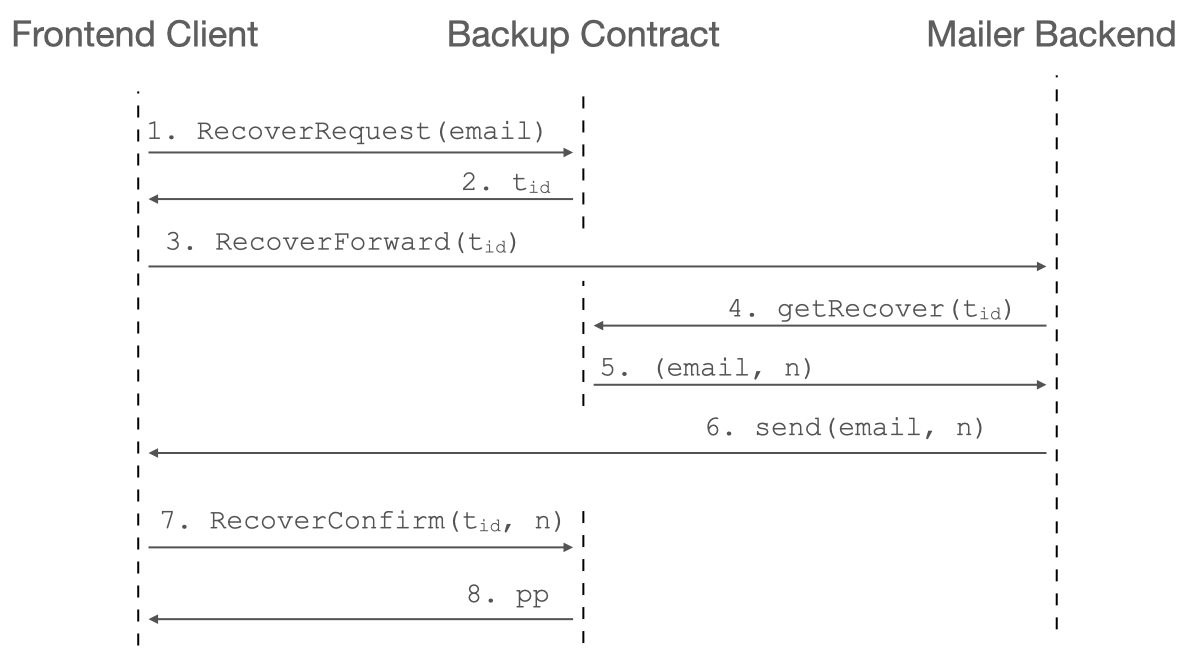
\includegraphics[width=\linewidth]{./media/media-002.png}
  \caption{Iteration 1 - Recovery}
  \label{it1:recovery}
\end{figure}

\begin{enumerate}
\item Alice enters her $email$ and, after pressing the submit button, a script running inside the webpage sends a transaction {\bf $\ms{recover}(email)$} to the Backup Contract to the Secret Network using a throwaway Secret wallet that Alice has just provisioned. 
\item The Backup Contract generates a transaction id $t_{id}$, a random confirmation code, stores the record $(t_{id}, email, code)$ in the {\tt recover} dataset, and returns the transaction id to Alice.
\item Alice forwards the transaction id to the Mailer Backend. 
\item The Mailer Backend queries the Backup Contract using that transaction id. 
\item The Backup Contract returns the email and confirmation code associated to the transaction id. 
\item The Mailer Backend sends the confirmation code to Alice by email. 
\item Alice opens her email and copies and pastes that verification code into her browser. After pressing the submit button, a script, running inside the webpage, sends a query $\ms{verify}(email, code)$ to the Backup Contract. 
\item The Backup Contract verifies the verification code, retrieves the corresponding record from the {\tt recover} dataset and returns the passphrase.
\end{enumerate}

\subsection{Security Analysis}

First and foremost, we are assuming that an attacker cannot retrieve data during transportation, storage, and execution without having the appropriate private keys thanks to the Secret Network protocol and the Intel SGX Trusted Execution Environment. That said, it is good to acknowledge that several attacks against Intel SGX have been published in the past few years \cite{gotzfried2017cache,nilsson2020survey,murdock2020plundervolt,biondo2018guard} but those vulnerabilities have been mitigated by the Secret Network. \\

First, the attacker could breach into Alice's mailbox or the Mailer Backend directly. During the backup phase, the attacker could use the confirmation code to upload an arbitrary passphrase for Alice. This is a problem if Alice recovers what she believes is her original passphrase but another that the attacker can access. Then, any new asset that Alice puts in her wallet can be stolen by the attacker from now. During the recovery phase it is even worst since the attacker could trigger and use the verification code to query the Backup Contract directly and get the passphrase back. \\

Secondly, the attacker could compromise either Alice's wallet or the Admin's wallet that was used to deploy the Backup Contract. In the case of Alice, it is recommended that she uses a throwaway Secret wallet when registering a passphrase as explained earlier. As soon as the passphrase has been recorded, she can forget about this wallet since she will not need it to recover her passphrase. However, if that wallet is compromised afterward, the attacker could look into the transaction history using that key and get Alice's passphrase. The same problem holds if the attacker can compromise the Admin's wallet. It is worse than compromising a single user's wallet since the attacker could retrieve all users' passphrases from the transaction history directly. 

\section{Iteration 2: Security Hardening}
\label{iteration2}

Our first iteration captures the right user experience but fails in terms of security. Two main security threats need to be addressed: 1) prevent the attacker from taking advantage of having access to emails and 2) prevent the attacker from recovering passphrase from compromised wallets. 

\subsection{The Secret NFT}

The first security problem is an authentication problem. Alice’s identity can be compromised if the attacker breaches into Alice’s mailbox, or worse, into the Mailer Backend directly. One way to prevent that is to add a second authentication factor. After careful consideration, we have chosen to rely on the blockchain directly. The idea is for Alice to store her passphrase in a Non-Fungible Token (NFT) \cite{wang2021non} during backup and transfer that NFT to her friend Charlie. When doomsday comes, Alice could recover her passphrase by asking Charlie to send that NFT back. With this solution, we are taking advantage of Secret Network NFTs that protect the confidentiality of its content and the privacy of its owners. This is an important security aspect since the attacker would not know who owns Alice's NFT.\\ 

Yet, one problem remains. When Charlie becomes the owner, he could access its content and Alice's passphrase. A solution to that is to have Alice encrypt her passphrase when minting the NFT so that Charlie cannot decrypt it without the key. However, we have another problem now, where to store the key when Alice needs it to recover her passphrase? We could adopt the same approach as described in iteration 1. Instead of storing all passphrases in the Backup Contract, we could store all users' encryption keys. 

\subsection{The Diffie-Hellman Key Exchange}

This Secret NFT solution helps us mitigate the second security issue as well. If the passphrase is never sent in clear to the network, the attacker cannot read it even if Alice's wallet or the Admin's wallet is compromised. The attacker could only retrieve the encryption key without being able to locate the encrypted content. For stronger security, we should prevent the attacker from getting that encryption key using a compromised wallet. This problem can be fixed implementing the {\em Diffie-Hellman Key Exchange} protocol to agree on the key without sharing it. The goal is to have Alice's wallet and the Backup Contract negotiate a key without exchanging it explicitly during the backup phase. The {\em Diffie–Hellman Key Exchange} protocol is a cryptography protocol that allows two parties, usually named Alice and Bob, that have no prior knowledge of each other, to securely agree on a shared key over an insecure channel \cite{diffie2022new}. That channel is considered as insecure because we assume that an attacker can eavesdrop on the communication and read all messages sent back and forth between Alice and Bob. \\

In practice, we use the {\em Elliptic-curve Diffie–Hellman} (abbreviated ECDH) that relies on Elliptic-curve cryptography \cite{bernstein2006curve25519}. In a nutshell, Alice generates an asymmetric key pair $(sec_A, pub_A)$ and sends the public one to Bob over the in-secure channel. When Bob receives Alice's public key, he will also generate its own pair $(sec_B, pub_b)$ and send his public key back to Alice. Once the public keys have been exchanged, Alice and Bob can combine the public key with their private key to generate the same shared secret value $s$. Alice computes $s=\ms{ECDH}(sec_A, pub_A, pub_B)$ and Bob computes the same shared secret value $s=\ms{ECDH}(sec_B, pub_B, pub_A)$. The security of the protocol resides in the fact that an attacker cannot compute that secret value $s$ even if $pub_A$ and $pub_B$ are known but not either $sec_A$ or $sec_B$. In practice, this shared secret value is usually not used as a cryptographic key directly. Instead, that shared value is given as input of a key derivation function such as the HMAC-based extract-and-expand key derivation function $\ms{HKDF}$ \cite{krawczyk2010hmac} that generates the same cryptographic key based on the secret value. 

\subsection{The Protocol}

Moreover, we are adding two additional features to our NFT-based Mnemonic Backup System. First, Alice can now back up several passphrases and still recover each of them with the same email. To do so, she will attach a unique id with each NFT during backup and ask for the Backup Contract for that specific id when she needs to recover the associated key. Secondly, Alice has now a limited time to enter her confirmation code during backup or validation code during recovery. This time limit is calculated based on the number of blocks that have been validated since Alice made her original request to the Backup Contract. \\

All of those new features are detailed in the new version of the protocol shown in figures \ref{it2:backup} and \ref{it2:recovery}. \\

{\bf Backup}

\begin{figure}[t]
  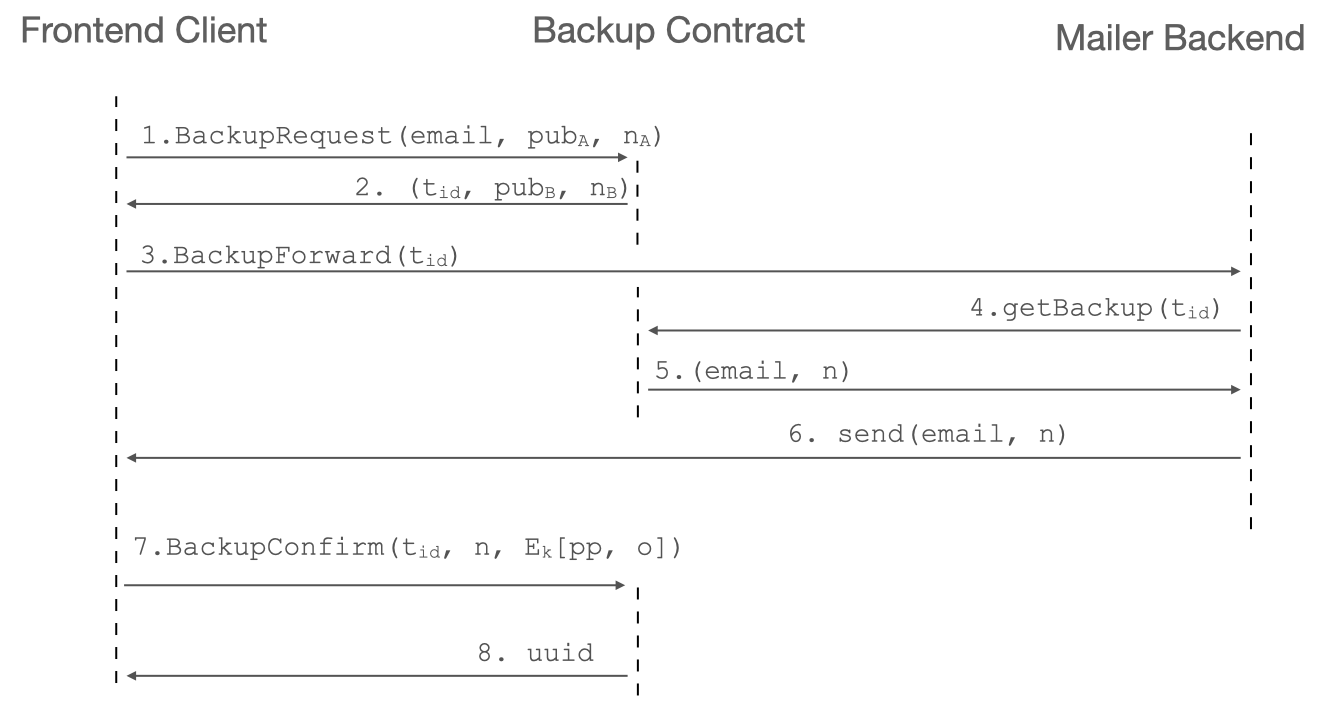
\includegraphics[width=\linewidth]{./media/media-003.png}
  \caption{Iteration 2 - Backup}
  \label{it2:backup}
\end{figure}

\begin{enumerate} 
\item Alice enters her $email$, her passphrase $m$, and an $id$ for her passphrase. After pressing the submit button, a script running inside the webpage generates an ECDH private and public key pair $(sec_A, pub_A)$, a nonce $n_A$, and sends the transaction $\ms{request}(email, id, pub_A, n_A)$ to the Secret Network using the throwaway Secret wallet that Alice has just provisioned.
\item The Backup Contract generates a transaction id $t_{id}$, a new ECDH private and public key pair $(sec_B, pub_B)$, and a nonce $n_B$. It calculates the ECDH secret $s=\ms{ECDH}(sec_B, pub_B, pub_A)$, and derives the 128-bit AES symmetric key $k$ using the standard password-based key derivation function $\ms{HKDF}$ and the concatenation of $n_A$ and $n_B$ as a salt $k=\ms{HKDF}(s, n_A || n_B)$. Finally, the contract stores the record $(email, id, t_{id}, b_{id}, pub_B, n_B)$ in the {\tt register} dataset and returns the transaction id to Alice.
\item Alice forwards the transaction id to the Mailer Backend. 
\item The Mailer Backend queries the Backup Contract $\ms{info}(t_id)$. 
\item The Backup Contract checks that the query comes from the Mailer Backend wallet's address, retrieves the record from the {\tt register} dataset, and checks that the query has not expired based on the initial block id $b_{id}$ and the current block id on the Secret Network. If not, it returns the $email$, the public key pair $pub_B$ and the nonce $n_B$ to the Mailer Backend. 
\item The Mailer Backend sends an email to Alice with the confirmation code $(pub_B, n_B)$. 
\item Alice opens her email and copies and pastes the confirmation code into her browser and enters her passphrase $pp$. After pressing the submit button, a script, running inside the webpage, calculates the ECDH secret $s=\ms{ECDH}(sec_A, pub_A, pub_B)$, and derives the AES symmetric key $k$ using $\ms{HKDF}$ and the concatenation of $n_A$ and $n_B$ as a salt $k=\ms{HKDF}(s, n_A || n_B)$. Then, it calculates a hash-based message authentication code (abbreviated HMAC) using the key $k$ and the concatenation of the email and id $h=\ms{HMAC}(k, email || id)$. Finally, the script sends the transaction $\ms{confirm}(t_{id}, h)$ to the Backup Contract. 
\item The Backup Contract checks that the query has not expired based on the initial block id $b_{id}$ and the current block id on the Secret Network. Then, it calculates the HMAC of the concatenation of the email and id using the key $h=\ms{HMAC}(k, email || id)$, and checks that this hash is strictly equal to the hash $h$ from the request. Finally, the contract stores the tuple $(email, id, k)$ in the {\tt confirm} dataset.
\item The client-side script can now encrypt (using AES in GCM mode) the passphrase $m$ with the key $k$ to obtain the ciphertext $c=E_{\ms{AES}}(k, m)$ and send the id and the ciphertext to the NFT contract.  
\item The NFT Contract mints a Secret NFT and returns the $NFT_{id}$.
\item Alice transfers the NFT to her friend Charlie. 
\end{enumerate}

{\bf Recovery}

\begin{figure}[t]
  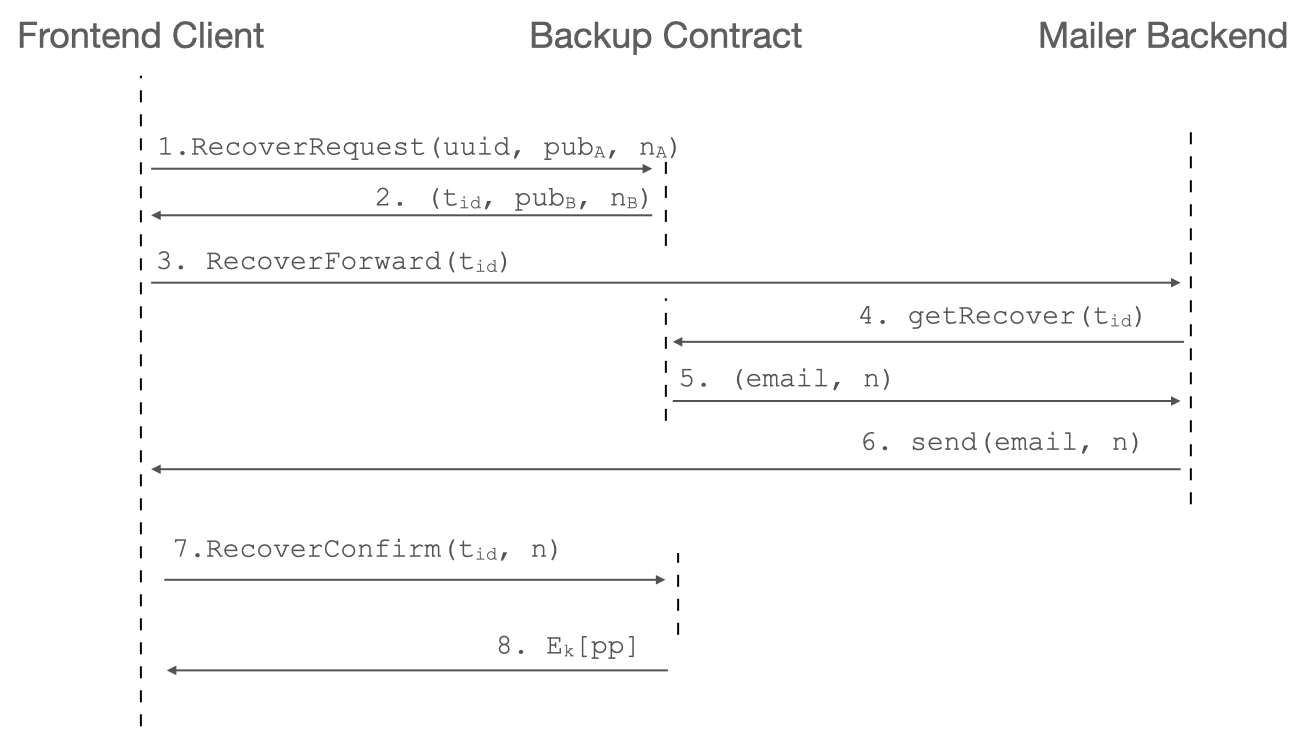
\includegraphics[width=\linewidth]{./media/media-004.png}
  \caption{Iteration 2 - Recovery}
  \label{it2:recovery}
\end{figure}

\begin{enumerate}
\item Alice creates a new Secret Wallet and asks Charlie to send her NFT back. Then, she goes to the recovery page that asks her to select the NFT id. A script running inside the webpage queries the NFT contract for that NFT id.  
\item The NFT contract returns the $id$ and the ciphertext from that NFT id.
\item The client's script generates a nonce $n_A$ and sends the transaction $\ms{request}(email, id, pub_A, n_A)$ to the Secret Network. 
\item The Backup Contract retrieves the record from the {\tt confirm} dataset using the email and id from the transaction. Then, it generates a nonce $n_B$ and stores the record $(email, id, t_{id}, b_{id}, n_B)$ in the {\tt register} dataset and returns the transaction id to Alice.
\item Alice forwards the transaction id to the Mailer Backend. 
\item The Mailer Backend queries the Backup Contract $\ms{info}(t_id)$. 
\item The Backup Contract checks that the query comes from the Mailer Backend wallet's address, retrieves the record from the {\tt register} dataset, and checks that the query has not expired based on the initial block id $b_{id}$ and the current block id on the Secret Network. If not, it returns the $email$, the public key pair $pub_B$, and the nonce $n_B$ to the Mailer Backend. 
\item The Mailer Backend sends an email to Alice with the confirmation code $(pub_B, n_B)$. 
\item Alice opens her email and copies and pastes that verification code into her browser. After pressing the submit button, a script, running inside the page, calculates the hash of the concatenation of the two nonces $h=\ms{H_{\ms{SHA512}}}(n_A || n_B)$. The script sends a query $\ms{verify}({email, id, h})$ to the Backup Contract. 
\item The Backup Contract checks that the query has not expired based on the initial block id $b_{id}$ and the current block id on the Secret Network. Then, it calculates the hash of the concatenation of the two nonces $h=\ms{H_{\ms{SHA512}}}(n_A || n_B)$ and checks that this hash is strictly equal to the hash $h$ from the request. Finally, it returns the key $k$ to the client. 
\end{enumerate}

Once the protocol is completed and Alice has received the key back, the client-side script can decrypt the ciphertext $c$ to obtain the passphrase $m=D_{\ms{AES}}(k, c)$. 

\subsection{Security Analysis}

Let's assume that the attacker can breach into Alice's mailbox or the Mailer Backend directly. During the backup phase, the attacker could not use the confirmation to upload an arbitrary key since the attacker does not know the client's id and the ECDH secret. During the recovery phase, the attacker could retrieve the encryption key but will not be able to get the passphrase without locating and getting the Secret NFT back first. \\

Let's assume that an attacker has compromised Alice's wallet or the Admin's wallet. The attacker would be able to locate the NFT but will have to 1) convince that person to send the NFTs back and 2) hijack the email to retrieve the encryption key. \\

In the end, carrying an attack is technically possible but way harder than in the first iteration. The attacker should first compromise one of the wallets to locate the NFT, convince the person holding the NFT to send it back to the attacker's wallet (phishing attack), and finally compromised the victim's email to retrieve the verification code.\\

However, having a friend holding the Secret NFT introduces another problem: what if that friend does not or cannot return the NFT? The passphrase would be locked forever. We are improving this availability issue in our next and final iteration. 

\section{Iteration 3: Improving Availability}
\label{iteration3}

Having a unique friend holding Alice's NFT can be a problem if that friend does not or cannot return it to her. A naive solution would be to duplicate the same NFT and send it to multiple friends. This solution is feasible but not ideal in terms of security since we are extending the attack surface. The attacker can now target multiple people to regain one of these NFTs. In this third and last iteration, we address the availability problem while preserving the security of our system by using {\em Shamir's Secret Sharing scheme}. 

\subsection{The Shamir's Secret Sharing Scheme}

Shamir's Secret Sharing scheme is a cryptography protocol usually used for splitting a secret into multiple parts, called shares, which individually do not give any information away about that secret \cite{shamir1979share}. To recover that secret, not all shares are needed but a minimum of shares that is called {\em ``the threshold''}. This is ideal from the usability perspective since the user does not have to collect all the shares back but only the minimum threshold required. Moreover, this is perfect from the security perspective since any attacker who can retrieve any number of shares less than the threshold will not be able to break the secret. \\

\subsection{The Protocol}

\begin{figure}[t]
  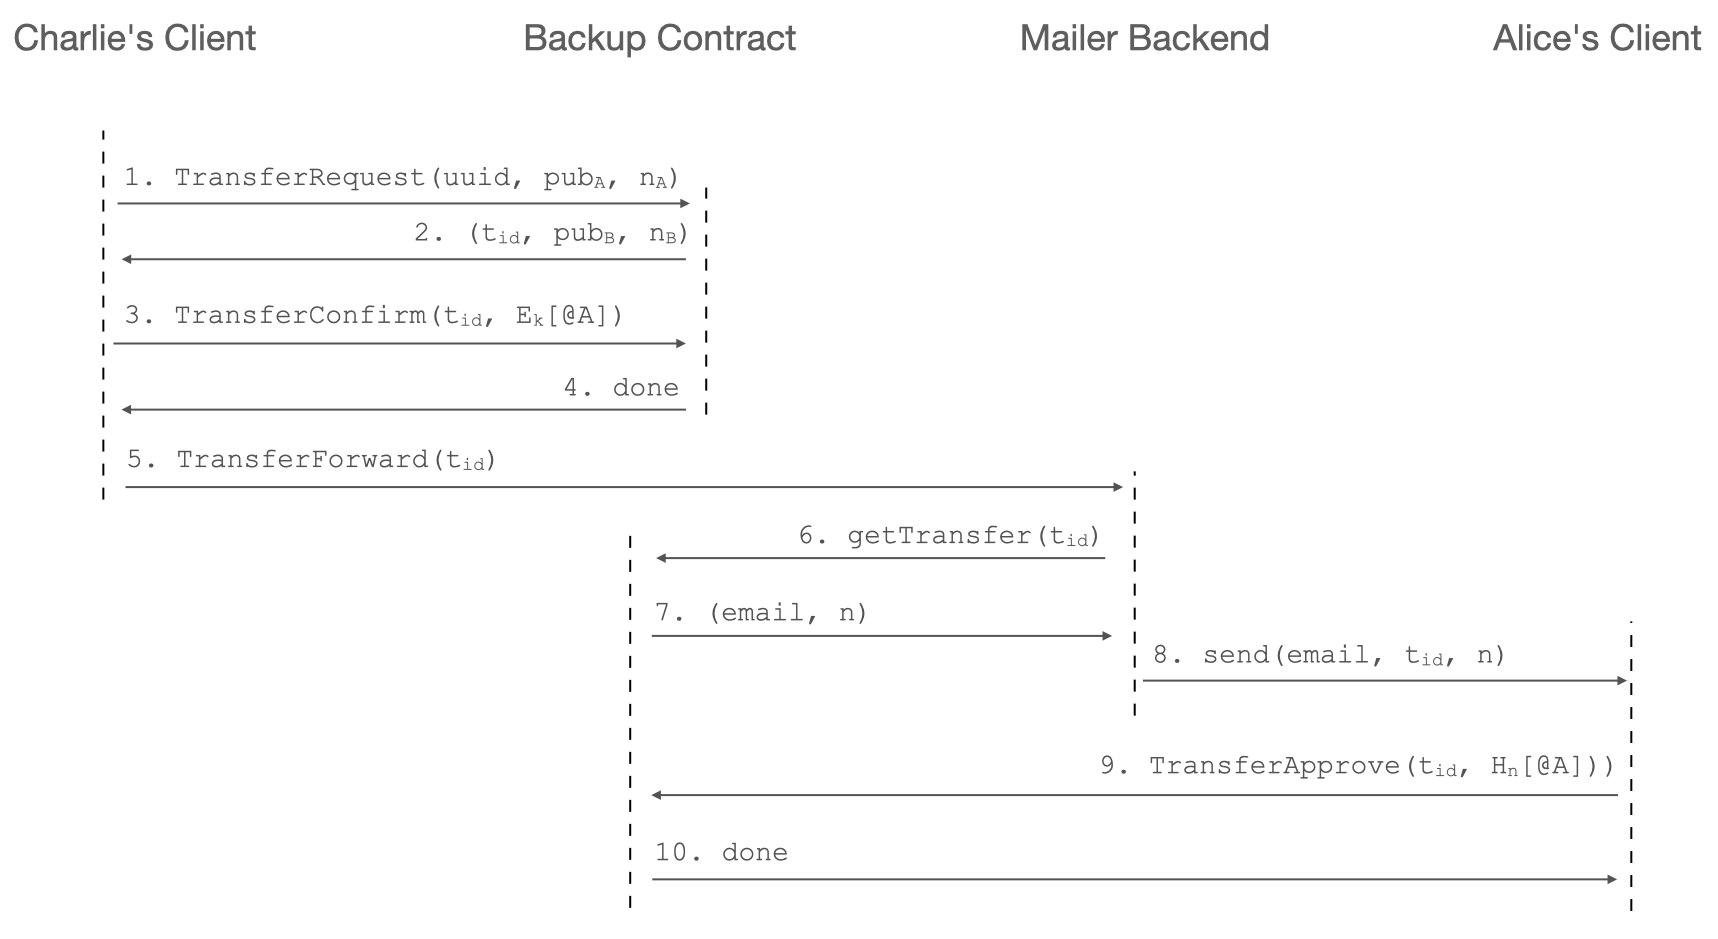
\includegraphics[width=\linewidth]{./media/media-005.png}
  \caption{Iteration 3 - Shamir's Secret Sharing NFTs}
  \label{it3:backup}
\end{figure}

{\bf For the backup}, Alice needs to specify the number of shares $i$ she wants to generate and the minimum number of shares $j$ needed to retrieve the passphrase (threshold value). Once, the encryption key has been fully registered in the contract, the script encrypts the passphrase, and concatenates the id and the ciphertext to generate the $i$ shares using the SSS algorithm: $(s_1,\cdots,s_i)=E_{\ms{SSS}}(id||c, i, j)$. Finally, the script mints the $i$ Secret NFTs on the Secret Network. Once the protocol is completed, Alice can now transfer the NFTs to her acquaintances. \\

{\bf For the recovery}, Alice creates a new Secret Wallet and asks all of her friends to send their NFTs back. Once she has at least $j$ of those NFTs in her wallet, she goes to the recovery page that asks her to select the NFTs. Then, the script in the webpage collects the shares and extracts the $id$ and the ciphertext from the NFTs $id||c = D_{\ms{SSS}}(s_1,\cdots,s_j)$. Then, the protocol continues like in the previous iteration. 

\section{Related Work}

Users must keep the wallet's mnemonic phrase safe because whoever gets access to that can access all of the crypto assets held in the wallet. To the best of our knowledge, there is only one significant proposal addressing the same issue. In \cite{rezaeighaleh2019new}, Rezaeighaleh and al. propose using a second wallet for backup. They propose a protocol based on Elliptic-Curve Diffie-Hellman to back up the private keys of the first wallet into a second wallet. They recommend having that secondary wallet be a ``cold'' wallet such as a hardware USB dongle or a smart card. This approach is technically sound but again relies on storing a physical object in a safe place which is hard in practice as shown in \cite{voskobojnikov2021u}. 

\section{Conclusion and Future Work}

In this paper, we propose a Decentralized Mnemonic Backup system that anyone can use to give custody of any blockchain passphrase to the Secret Network and recover it using a simple email. The idea is to encrypt the passphrase and split it into multiple Secret NFTs using {\em Shamir's Secret Sharing} cryptographic protocol. The encryption key is saved in a Secret smart contract. This key is never recorded in any transaction. Instead, it is generated using the {\em Diffie-Hellman Key Exchange} protocol which is similarly used in well-known protocols such as TLS and the {\em Signal} messaging app. \\

The key recovering system can be used outside of our Mnemonic Backup system. It can be used for more advanced cryptographic protocols that involve storing and managing secret keys on-chain with the option of recovering them using an email. For instance, this can be used to encrypt files on the InterPlanetary File System
(IPFS) \cite{muralidharan2019interplanetary} and manage the access using a Secret Contract that would hold custody of the encryption key. Our system could be used to safely generate and manage the encryption key on the Secret Network and possibly have an email backup solution if such a feature is desired.  

\subsubsection{Acknowledgments} This work has been funded through a grant from the {\em Secret Network}. We want to thank the people from {\em Secret Labs} for giving us early feedback on our proposal and helping us develop the prototype. 

\bibliographystyle{splncs04}
\bibliography{whitepaper}

\end{document}
